\documentclass[11pt]{article}
\usepackage[T1]{fontenc}
\usepackage{lmodern}
\usepackage[margin=1in]{geometry}
\usepackage{amsmath,amssymb,amsthm}
\usepackage{booktabs}
\usepackage{tikz}
\usepackage{fancyvrb}
\usepackage[hidelinks]{hyperref}
\usepackage{xurl}

\newtheorem{theorem}{Theorem}
\newtheorem{lemma}[theorem]{Lemma}
\newtheorem{conjecture}[theorem]{Conjecture}
\theoremstyle{remark}
\newtheorem{remark}[theorem]{Remark}

\newcommand{\RC}{\mathrm{RC}}
\newcommand{\tmax}{t_{\max}}

\title{The Odd Sum conjecture for Roller Coaster permutations fails at $n = 17$}
\author{Qianghao Wu}
\date{November 28, 2026}

\begin{document}
\maketitle

\begin{abstract}
For a permutation $\pi$ of $\{1,\dots,n\}$, let $t(\pi)$ be the total number of maximal increasing and maximal decreasing runs, summed over all subsequences of $\pi$ with at least three entries. A Roller Coaster permutation is a permutation with the largest value of $t$. Ahmed and Snevily (2013) conjectured that every Roller Coaster permutation of odd length $n = 2k+1$ has the Odd Sum property: $\pi_j + \pi_{n-j+1}$ is odd for $1 \le j \le k$. We show that this conjecture is false for $n = 17$. The permutation $8, 14, 3, 15, 6, 10, 2, 17, 7, 12, 1, 16, 5, 11, 4, 13, 9$, found by Botler and Netto with integer linear programming, has $t = 798783$, and two of its eight mirror sums are even. An exact exhaustive search shows that every permutation of $\{1,\dots,17\}$ with the Odd Sum property has $t \le 798775$. A second exact search gives $\tmax(17) = 798783$ and shows that the Roller Coaster permutations of length 17 are 128 permutations, none with the Odd Sum property. Netto's 2022 thesis already reports $\tmax(17) = 798783$ with this permutation, from a floating-point solver; we found no source that notes the failure of the conjecture. Lean 4 with Mathlib proves the value $t = 798783$ from the definition, and it proves that the bound for Odd Sum permutations implies the failure. The bound itself is a computation outside Lean; two separately written programs give the same result. We also show that the conjecture holds for $n \le 16$. This work has not yet been reviewed by experts. The computations, the proofs and the text were produced by AI models (from Anthropic and OpenAI), working under the author's direction.
\end{abstract}

\section{Introduction}

A permutation $\pi$ of $[n] = \{1, 2, \dots, n\}$ is a sequence $(\pi_1, \dots, \pi_n)$, and $S_n$ is the set of these permutations. Ahmed and Snevily~\cite{AS} define, for a sequence $\tau$ of distinct numbers, $i(\tau)$ and $d(\tau)$ as the numbers of increasing and decreasing ``sequences of contiguous numbers'' in $\tau$, where such a sequence has at least two numbers, and $\mathrm{id}(\tau) = i(\tau) + d(\tau)$. Their examples $\mathrm{id}(2143) = 3$ and $\mathrm{id}(1234) = 1$ show that these sequences are the maximal monotone runs of consecutive entries. With $X(\pi)$ the set of subsequences of $\pi$ with at least three entries,
\[
  t(\pi) = \sum_{\tau \in X(\pi)} \mathrm{id}(\tau).
\]
For example, $t(2143) = 11$ and $t(1234) = 5$. A permutation $\pi \in S_n$ is a \emph{Roller Coaster permutation} if $t(\pi) = \max_{\sigma \in S_n} t(\sigma)$. We write $\RC(n)$ for the set of these permutations and $\tmax(n)$ for the maximum. The reverse and the complement $\pi^* = (n+1-\pi_1, \dots, n+1-\pi_n)$ of a permutation in $\RC(n)$ are in $\RC(n)$~\cite{AS}.

Ahmed and Snevily computed $\RC(n)$ for $n \le 13$, gave a construction that bounds $\tmax(n)$ from below for $n \le 24$, and stated five conjectures. One of them is the following.

\begin{conjecture}[Ahmed and Snevily~{\cite[Conjecture 2.4]{AS}}, the Odd Sum conjecture]\label{conj:oddsum}
``If $\pi \in \RC(n)$ and $n = 2k + 1$, then $\pi_j + \pi_{n-j+1}$ is odd for $1 \le j \le k$. If $\pi \in \RC(n)$ and $n = 2k$, then $\pi_j + \pi_{n-j+1} = 2k + 1$ for all $1 \le j \le k$.''
\end{conjecture}

The Open Problem Garden lists the conjecture in the entry ``Roller Coaster permutations''~\cite{OPG}, together with the conjecture on $|\RC(n)|$ (\cite[Conjecture 2.3]{AS}). For odd $n$ we say that a permutation has the \emph{Odd Sum property} if $\pi_j + \pi_{n-j+1}$ is odd for $1 \le j \le (n-1)/2$; we call these $(n-1)/2$ numbers the \emph{mirror sums} of $\pi$.

\paragraph{Earlier work.}
Ahmed and Snevily~\cite{AS} give $\tmax(n)$ for $3 \le n \le 13$ and lower bounds for $14 \le n \le 24$; for $n = 17$ their bound is $\tmax(17) \ge 798471$. Their construction for odd $n$ puts the values $k$ and $k+1$ at the ends; their permutation for $n = 17$ has the Odd Sum property. Adamczak~\cite{Ad1} studies the structure of $\RC(n)$: he gives a proof that the first and last entries of a Roller Coaster permutation differ by one, and he writes that this result ``will be used in building up to the proof of the odd-sums conjecture''. He also introduces recursively alternating permutations. Botler and Netto~\cite{BN} give an $O(n^3)$ formula for $t$ and an integer linear program for Roller Coaster permutations. They solve it with Gurobi and report new lower bounds for $\tmax(n)$, $n \le 40$. For $n = 17$ their Table~1 lists the permutation
\[
  w = (8, 14, 3, 15, 6, 10, 2, 17, 7, 12, 1, 16, 5, 11, 4, 13, 9).
\]
Netto's master's thesis~\cite{Netto} repeats this permutation (Table 2.1) and states, for the model without extra constraints, that ``these results are indeed optimal. In particular, the value $\tmax(17) = 798783$ shows an improvement on the lower bound given by T. Ahmed and H. Snevily''. This is a floating-point solver result without a certificate. Neither~\cite{BN} nor~\cite{Netto} mentions the Odd Sum conjecture. Adamczak's revised note on partition numbers~\cite{Ad2} (version 2, December 2025) discusses the work of Netto and of Botler and Netto. It does not mention a failure of the Odd Sum conjecture. We found no source that notes that $w$ breaks the conjecture.

\paragraph{Result.}
The mirror sums of $w$ are $17, 27, 7, 26, 11, 26, 3, 29$. The sums for $j = 4$ and $j = 6$ are even (Figure~\ref{fig:witness}).

\begin{theorem}\label{thm:main}
The Odd Sum conjecture is false for $n = 17$. More precisely:
\begin{enumerate}
\item[(i)] $t(w) = 798783$, and $w$ does not have the Odd Sum property;
\item[(ii)] every permutation of $[17]$ with the Odd Sum property has $t \le 798775$;
\item[(iii)] $\tmax(17) = 798783$ and $|\RC(17)| = 128$; no element of $\RC(17)$ has the Odd Sum property.
\end{enumerate}
\end{theorem}

Facts (i) and (ii) are enough: by (i), $\tmax(17) \ge 798783$, and by (ii) no Odd Sum permutation reaches this value. Since $S_{17}$ is finite, $\RC(17)$ is not empty, and each of its elements breaks the conjecture. Fact (iii) is stronger than needed and describes $\RC(17)$ completely.

\paragraph{What is new.}
The permutation $w$ is due to Botler and Netto~\cite{BN}, who report $t(w)$ as a lower bound. The statement $\tmax(17) = 798783$ is due to Netto~\cite{Netto}, from a solver run without a certificate. New in this paper are: the observation that the Odd Sum conjecture fails at $n = 17$; exact proofs of (i), (ii) and (iii), with the value of $t(w)$ and the logical step checked in Lean; the complete set $\RC(17)$; and exact checks that the conjecture holds for $n \le 16$ (Section~\ref{sec:small}).

\begin{figure}[t]
\centering
% Generated by checks/draw_witness.py; do not edit.
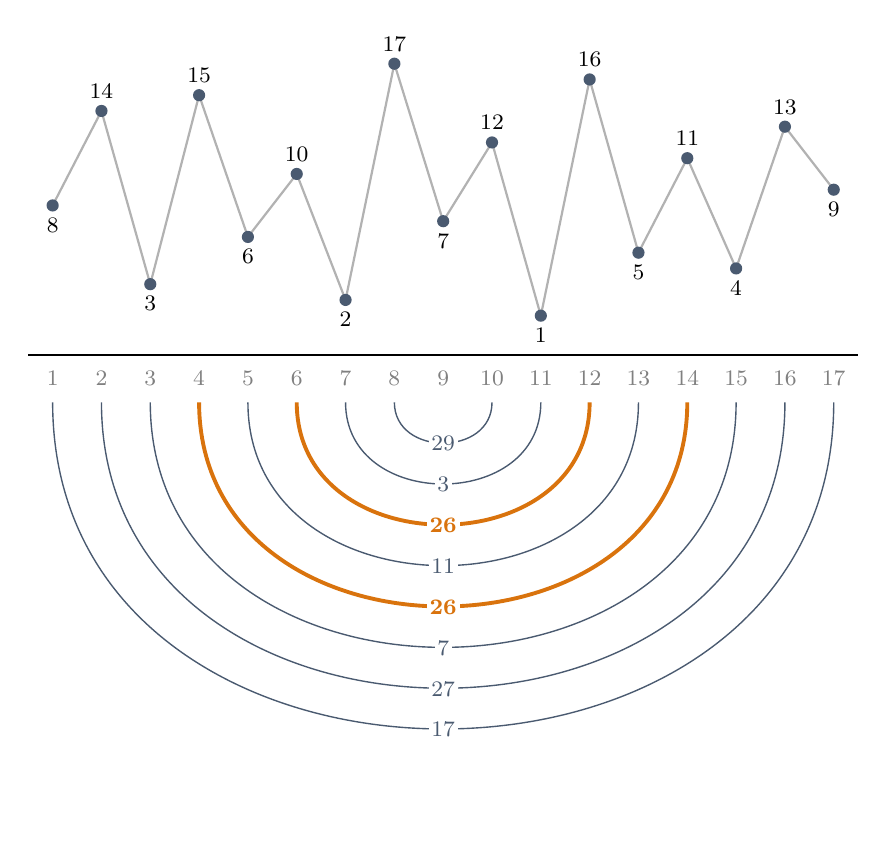
\begin{tikzpicture}[x=0.62cm,y=0.2cm,font=\footnotesize]
\definecolor{oddc}{HTML}{4A5A70}\definecolor{evenc}{HTML}{D9730D}
\draw[gray!60,line width=0.8pt] (1,8) -- (2,14) -- (3,3) -- (4,15) -- (5,6) -- (6,10) -- (7,2) -- (8,17) -- (9,7) -- (10,12) -- (11,1) -- (12,16) -- (13,5) -- (14,11) -- (15,4) -- (16,13) -- (17,9);
\fill[oddc] (1,8) circle (2.2pt) node[below=1pt,black] {8};
\fill[oddc] (2,14) circle (2.2pt) node[above=1pt,black] {14};
\fill[oddc] (3,3) circle (2.2pt) node[below=1pt,black] {3};
\fill[oddc] (4,15) circle (2.2pt) node[above=1pt,black] {15};
\fill[oddc] (5,6) circle (2.2pt) node[below=1pt,black] {6};
\fill[oddc] (6,10) circle (2.2pt) node[above=1pt,black] {10};
\fill[oddc] (7,2) circle (2.2pt) node[below=1pt,black] {2};
\fill[oddc] (8,17) circle (2.2pt) node[above=1pt,black] {17};
\fill[oddc] (9,7) circle (2.2pt) node[below=1pt,black] {7};
\fill[oddc] (10,12) circle (2.2pt) node[above=1pt,black] {12};
\fill[oddc] (11,1) circle (2.2pt) node[below=1pt,black] {1};
\fill[oddc] (12,16) circle (2.2pt) node[above=1pt,black] {16};
\fill[oddc] (13,5) circle (2.2pt) node[below=1pt,black] {5};
\fill[oddc] (14,11) circle (2.2pt) node[above=1pt,black] {11};
\fill[oddc] (15,4) circle (2.2pt) node[below=1pt,black] {4};
\fill[oddc] (16,13) circle (2.2pt) node[above=1pt,black] {13};
\fill[oddc] (17,9) circle (2.2pt) node[below=1pt,black] {9};
\draw (0.5,-1.5) -- (17.5,-1.5);
\foreach \j in {1,...,17} \node[gray] at (\j,-3) {\j};
\draw[oddc,line width=0.5pt] (1,-4.5) .. controls (1,-32.16) and (17,-32.16) .. (17,-4.5);
\node[oddc,fill=white,inner sep=1pt] at (9,-25.30) {17};
\draw[oddc,line width=0.5pt] (2,-4.5) .. controls (2,-28.71) and (16,-28.71) .. (16,-4.5);
\node[oddc,fill=white,inner sep=1pt] at (9,-22.70) {27};
\draw[oddc,line width=0.5pt] (3,-4.5) .. controls (3,-25.25) and (15,-25.25) .. (15,-4.5);
\node[oddc,fill=white,inner sep=1pt] at (9,-20.10) {7};
\draw[evenc,line width=1.4pt] (4,-4.5) .. controls (4,-21.79) and (14,-21.79) .. (14,-4.5);
\node[evenc,fill=white,inner sep=1pt] at (9,-17.50) {\textbf{26}};
\draw[oddc,line width=0.5pt] (5,-4.5) .. controls (5,-18.33) and (13,-18.33) .. (13,-4.5);
\node[oddc,fill=white,inner sep=1pt] at (9,-14.90) {11};
\draw[evenc,line width=1.4pt] (6,-4.5) .. controls (6,-14.87) and (12,-14.87) .. (12,-4.5);
\node[evenc,fill=white,inner sep=1pt] at (9,-12.30) {\textbf{26}};
\draw[oddc,line width=0.5pt] (7,-4.5) .. controls (7,-11.42) and (11,-11.42) .. (11,-4.5);
\node[oddc,fill=white,inner sep=1pt] at (9,-9.70) {3};
\draw[oddc,line width=0.5pt] (8,-4.5) .. controls (8,-7.96) and (10,-7.96) .. (10,-4.5);
\node[oddc,fill=white,inner sep=1pt] at (9,-7.10) {29};
\end{tikzpicture}

\caption{The witness $w$. Top: the points $(j, w_j)$. Bottom: an arc joins the mirror positions $j$ and $18-j$ and carries the mirror sum $w_j + w_{18-j}$. The sums at $j = 4$ and $j = 6$ (orange) are even.}
\label{fig:witness}
\end{figure}

\section{Two tools}

Positions in this section are $1, \dots, n$. For positions $a < b < c$, the triple $(a, b, c)$ is a \emph{turn} of $\pi$ if $\pi_b$ is larger than both $\pi_a$ and $\pi_c$ or smaller than both.

\begin{lemma}[turn identity]\label{lem:turn}
For $\pi \in S_n$,
\[
  t(\pi) = \sum_{m=3}^{n} \binom{n}{m} + \sum_{\substack{a<b<c\\ (a,b,c) \text{ a turn}}} 2^{a-1}\, 2^{n-c}.
\]
\end{lemma}

\begin{proof}
Let $\tau$ have $m \ge 2$ distinct entries. The $m-1$ comparisons of adjacent entries form maximal blocks of equal direction, and $\mathrm{id}(\tau)$ is the number of blocks. The number of blocks is one more than the number of interior entries where the direction changes, that is, the interior entries that are larger or smaller than both neighbours in $\tau$. So $\mathrm{id}(\tau) = 1 + (\text{number of turns of } \tau \text{ at consecutive entries})$. Sum over $\tau \in X(\pi)$. The first term gives $|X(\pi)| = \sum_{m \ge 3} \binom{n}{m}$. A turn $(a, b, c)$ of $\pi$ is a turn at consecutive entries of $\tau$ exactly when $\tau$ contains the positions $a, b, c$ and no position strictly between $a$ and $c$ other than $b$. The other positions are free: $2^{a-1}$ choices before $a$ and $2^{n-c}$ choices after $c$.
\end{proof}

This is the same formula as the one of Botler and Netto~\cite[Section 2]{BN}, who group the turns (their ``triangles'') by $c - a + 1$. With $W = \sum_{a < c} (c - a - 1)\, 2^{a-1} 2^{n-c}$, the weight of all triples, we have $t(\pi) = \sum_{m \ge 3}\binom{n}{m} + W - L(\pi)$, where the \emph{loss} $L(\pi)$ is the total weight of the triples that are not turns (the monotone triples). Both search programs below bound $L$ from below.

\begin{lemma}\label{lem:sym}
The complement $\pi \mapsto \pi^*$ keeps $t$ and keeps the Odd Sum property.
\end{lemma}

\begin{proof}
The complement reverses every comparison, so it keeps the set of turns, and Lemma~\ref{lem:turn} gives $t(\pi^*) = t(\pi)$. The mirror sums change from $s$ to $2(n+1) - s$, which has the same parity.
\end{proof}

So it is enough to search the permutations with $\pi_1 \le (n+1)/2$; the complements give the others.

\section{Fact (i) and the Lean statement}\label{sec:lean}

We checked $t(w) = 798783$ in three ways: in Lean from the definition, in Python from the definition (all $2^{17}$ subsequences), and in Python from Lemma~\ref{lem:turn}.

The Lean file \path{lean/Solution.lean} imports only Mathlib. It states the definitions of Ahmed and Snevily directly: \texttt{idv} counts the maximal blocks of the list of adjacent comparisons; \texttt{tval} sums \texttt{idv} over the sublists of length at least 3 (\texttt{List.sublists}); \texttt{IsRC n $\pi$} says that the list $\pi$ is a permutation of $[1, \dots, n]$ and that $\mathtt{tval}\,\sigma \le \mathtt{tval}\,\pi$ for every such $\sigma$; and \texttt{OddSumConjecture n} is Conjecture~\ref{conj:oddsum} for one $n$, with $\pi_j$ read as the entry with index $j - 1$. Lean proves the source's examples $\mathrm{id}(2143) = 3$, $\mathrm{id}(1234) = 1$, $t(2143) = 11$ and $t(1234) = 5$ for these definitions. The two main theorems are:
\begin{Verbatim}[fontsize=\small,commandchars=\\\{\}]
theorem fact_i : witness.Perm (List.range' 1 17) \(\wedge\) tval witness = 798783 \(\wedge\)
    witness.getD 3 0 + witness.getD 13 0 = 26

theorem not_oddSumConjecture_17
    (h : \(\forall\) \(\sigma\) : List \(\mathbb{N}\), \(\sigma\).Perm (List.range' 1 17) \(\to\) OddSum17 \(\sigma\) \(\to\) tval \(\sigma\) < 798783) :
    \(\neg\) OddSumConjecture 17
\end{Verbatim}
Here \texttt{OddSum17 $\sigma$} says that $\sigma_j + \sigma_{18-j}$ is odd for $1 \le j \le 8$. The hypothesis \texttt{h} of the second theorem is fact (ii) in a weaker form. \textbf{Lean does not prove fact (ii)}; Section~\ref{sec:search} proves it by computation. So the Lean part of the result is: the value of $t(w)$ from the definition, and the step from (i) and (ii) to the failure of the conjecture.

The value $t(w)$ is a sum over $2^{17}$ sublists. One kernel evaluation of the definition did not finish within 6\,GB of memory. The file proves a lemma that rewrites \texttt{tval} as a binary recursion over the list, splits the sum into 32 parts by the sublist of the first five entries, and evaluates each part with \texttt{decide +kernel}. No \texttt{native\_decide} is used. \texttt{\#print axioms} gives \texttt{[propext, Classical.choice, Quot.sound]} for both theorems, and \texttt{lake comparator} confirms that the file proves exactly the statements of \path{lean/Challenge.lean}.

\section{Fact (ii): the exact search}\label{sec:search}

\paragraph{Method.}
The program \path{checks/oddsum_bb.c} places the values position by position from left to right. It uses only integer arithmetic. In the Odd Sum mode, a value at position $j > 9$ must have the parity opposite to the value at position $18 - j$, and the middle value must be odd (there are nine odd and eight even values, and the Odd Sum property pairs the other sixteen positions into eight odd--even pairs). A branch is cut only when a lower bound on the final loss $L$ is larger than $\sum_m \binom{n}{m} + W - T$, that is, when every completion has $t < T$. The lower bound is the sum of four parts, over disjoint sets of triples:
\begin{enumerate}
\item triples with all three positions placed: their exact loss;
\item triples with the first two positions placed: the loss depends only on the value at the third position;
\item triples with only the first position placed: for each free position $q$ and value $v$ at $q$, the loss is at least $\min(\ell, h)(2^{n-q} - 1)$, where $\ell$ and $h$ are the weights of the placed positions with smaller and larger values than $v$;
\item triples with no position placed: at least $2^{n-m}$ times the minimum loss over $S_m$, where $m$ is the number of free positions.
\end{enumerate}
Parts 2 and 3 depend on which value goes to which free position. The program bounds their sum by the rearrangement inequality: it pairs the smallest per-value cost with the largest position weight. When every free position has a forced parity, it pairs inside each parity class. The minimum losses for part 4 are computed exactly by the same program for $m \le 12$; for $m > 12$ the program uses $2 \cdot (\text{value for } m - 1)$, which is a valid lower bound because deleting the last position keeps every other triple and halves its weight. The comments of the program give each step. The search fixes $\pi_1 \le 9$ (Lemma~\ref{lem:sym}). It runs as four independent processes that split the tree at depth 2.

\paragraph{Result.}
With $T = 798775$ the program lists every Odd Sum permutation with $t \ge 798775$ and $\pi_1 \le 9$. It finds 96 permutations, all with $t = 798775$, and nothing larger. The four processes visit $893\,550\,028$, $893\,260\,703$, $910\,073\,485$ and $841\,092\,770$ nodes, and each took between 943 and 1030 seconds on one core of a Steam Deck (AMD Zen~2). With their complements there are 128 Odd Sum permutations with $t = 798775$, and every Odd Sum permutation of $[17]$ has $t \le 798775$. This is fact (ii). The maximum over Odd Sum permutations, 798775, is larger than the lower bound 798471 of Ahmed and Snevily, whose permutation for $n = 17$ has the Odd Sum property.

\paragraph{A second program.}
The program \path{checks/independent/v2_bb.c} was written separately, by a different AI model, before its author read \texttt{oddsum\_bb.c}. It uses the same idea: the loss $L$, the same kinds of lower bound, the rearrangement inequality and the complement symmetry. It differs in the details: it uses no parity classes and no forced middle parity, it computes the minimum losses for $m \le 12$ by itself (without the values of~\cite{AS}), and it splits the search by the value of $\pi_1$. For fact (ii) it visits $8.7 \cdot 10^9$ nodes and lists the same 96 permutations. The two programs share the method, so an error in the method would affect both; a coding error in one of them would show as a difference.

\paragraph{Validation.}
Both programs were compared with brute force over all permutations: \texttt{oddsum\_bb} for $n = 5, \dots, 10$, in both modes and at four thresholds each (36 sets of permutations, all equal), and \texttt{v2\_bb} for $n = 5, \dots, 9$ at five thresholds (50 sets, all equal). The brute force uses Lemma~\ref{lem:turn}, which is checked against the definition on random permutations for $n \le 8$ and on all permutations for $n \le 7$. Every permutation that a search lists is evaluated again in Python.

\section{Fact (iii) and small $n$}\label{sec:small}

The same program without the Odd Sum rows and with $T = 798783$ lists every permutation of $[17]$ with $t \ge 798783$ and $\pi_1 \le 9$. It finds 96 permutations, all with $t = 798783$ (four processes, $3.96 \cdot 10^{10}$ nodes in total, between 11\,957 and 12\,542 seconds each on one core). The second program gives the same 96 permutations. With the complements, $|\mathrm{RC}(17)| = 128$ and $\tmax(17) = 798783$, as Netto found with Gurobi~\cite{Netto}. This confirms his value exactly.

The set $\RC(17)$ has the following properties; each one is checked by \path{checks/check_lists.py}.
\begin{itemize}
\item No element has the Odd Sum property. In every element, the even mirror sums are exactly those at $j = 4$ and $j = 6$.
\item $\RC(17)$ is closed under reversal and complement. It contains $w$.
\item Every element is alternating or reverse-alternating, so Conjecture~2.1 of~\cite{AS} holds at $n = 17$. Every element has $|\pi_1 - \pi_{17}| = 1$, as Adamczak's theorem~\cite{Ad1} requires. Exactly 32 elements have $\pi_1 = 8$ and $\pi_{17} = 9$, so Conjecture~2.2 of~\cite{AS} holds at $n = 17$.
\item $|\RC(17)| = 128 = 2^7 \le 2^{9}$, as Conjecture~2.3 of~\cite{AS} predicts.
\item Ahmed and Snevily define $g_L(\pi)$ by swapping $\pi_i$ and $\pi_{n-i+1}$ for each $i \in L \subseteq \{1, \dots, k\}$, and $g(\pi)$ as the set of these permutations and their complements~\cite[Section 2]{AS}. The set $g(w)$ has 512 elements, and its elements with the largest $t$ are exactly $\RC(17)$. This agrees with the description of $\RC(2k+1)$ that Ahmed and Snevily give after Conjecture~2.5.
\end{itemize}

\paragraph{Smaller $n$.}
Table~\ref{tab:small} gives exact values of $\tmax(n)$ and $|\RC(n)|$. For $n \le 14$ they come from an earlier exact search of this project (\path{checks/rc4.c}, with a weaker bound); its output is in \path{data/logs}. For $n = 15$ and $n = 16$ they come from \path{checks/run_rc.py}, which runs the unrestricted search of both programs. For $n \le 13$ the values agree with~\cite{AS}. For $n = 14, 15, 16$ they agree with the lower bounds of~\cite{AS} and with the values of Netto~\cite{Netto}, and they are now exact. For every $n \le 16$, every element of $\RC(n)$ satisfies Conjecture~\ref{conj:oddsum}. So $n = 17$ is the smallest $n$ for which the conjecture fails.

\begin{table}[t]
\centering
\begin{tabular}{rrr}
\toprule
$n$ & $\tmax(n)$ & $|\RC(n)|$ \\
\midrule
3 & 2 & 4 \\
4 & 11 & 4 \\
5 & 37 & 8 \\
6 & 106 & 4 \\
7 & 270 & 16 \\
8 & 653 & 4 \\
9 & 1523 & 32 \\
10 & 3480 & 4 \\
11 & 7768 & 64 \\
12 & 17123 & 4 \\
13 & 37405 & 64 \\
14 & 81350 & 4 \\
15 & 174954 & 128 \\
16 & 374409 & 4 \\
17 & 798783 & 128 \\
\bottomrule
\end{tabular}
\caption{Exact values. The conjecture holds for $n \le 16$ and fails for $n = 17$.}
\label{tab:small}
\end{table}

\section{How the result was checked}

\begin{itemize}
\item Lean: \texttt{lake env lean lean/Solution.lean} on Lean v4.36.0 and Mathlib v4.36.0 (about 8 minutes, up to 6\,GB of memory), \texttt{\#print axioms}, and \texttt{lake comparator} against \path{lean/Challenge.lean}. \texttt{Challenge.lean} repeats the definitions and the two statements of Section~\ref{sec:lean}; a reader must compare it with Conjecture~\ref{conj:oddsum}.
\item Searches: both programs, for fact (ii) and for $n = 15$ (\path{checks/run_n17.py}, \path{checks/run_rc.py}); the runs for fact (iii) and for $n = 16$ are recorded in \path{data/logs}.
\item The script \path{checks/ci.sh} repeats everything except Lean, the unrestricted runs for $n = 16$ and $n = 17$, and the search for $n \le 14$. It compares every count with \path{data/expected.json} and with this text.
\item Before this paper was written, a separate verification stage reran the Lean checks and both searches for fact (ii), wrote the second program, and compared the lists.
\end{itemize}

\section{Limits}

\begin{enumerate}
\item Fact (ii) is a computation. Lean does not check it. Its correctness rests on the lower bound of Section~\ref{sec:search} and on two programs that share the method.
\item The programs were compared with brute force only for $n \le 10$ (\texttt{oddsum\_bb}) and $n \le 9$ (\texttt{v2\_bb}).
\item The results for $n = 15$ and $n = 16$ were computed while this paper was written. A later recheck reran both searches, with both programs, on a clean copy and got the same lists.
\item We settle the conjecture only by one counterexample length. For other $n \ge 18$, odd or even, we do not know if the conjecture holds. In Table~1 of Botler and Netto~\cite{BN}, the permutations for $n = 25, 33, 35, 37, 38, 39, 40$ break the condition of the conjecture, but for $n \ge 18$ their model has extra constraints, so these permutations are not known to be in $\RC(n)$.
\end{enumerate}

\section*{Software and data}
The Lean proof uses Lean~4 (\url{https://lean-lang.org}) and Mathlib (\url{https://github.com/leanprover-community/mathlib4}). The programs, the logs and the lists of permutations are in the folders \path{checks/} and \path{data/} next to this paper.

\begin{thebibliography}{9}

\bibitem{Ad1}
W.~L. Adamczak, \emph{A note on the structure of Roller Coaster permutations}, arXiv:1605.02415, 2016. \url{https://arxiv.org/abs/1605.02415}

\bibitem{Ad2}
W.~Adamczak, \emph{Roller coaster permutations and partition numbers}, arXiv:1703.08735v2, December 29, 2025. \url{https://arxiv.org/abs/1703.08735v2}

\bibitem{AS}
T.~Ahmed and H.~Snevily, \emph{Some properties of Roller Coaster permutations}, Bull. Inst. Combin. Appl.\ (2013). Preprint: \url{https://tanbir.github.io/files/preprints/ahmed_snevily_roller_coaster_permutations.pdf}

\bibitem{BN}
F.~Botler and B.~L. Netto, \emph{New bounds on Roller Coaster permutations}, in: Anais do VI Encontro de Teoria da Computa\c{c}\~ao (ETC), SBC, 2021, pp.~50--53. \href{https://doi.org/10.5753/etc.2021.16378}{doi:10.5753/etc.2021.16378}

\bibitem{Netto}
B.~R.~L. Netto, \emph{Two Problems in Combinatorics: Roller Coaster Permutations \& the Erd\H{o}s--S\'os Conjecture}, master's thesis, COPPE, Universidade Federal do Rio de Janeiro, March 2022. \url{https://pesc.coppe.ufrj.br/uploadfile/publicacao/3043.pdf}

\bibitem{OPG}
T.~Ahmed and H.~S. Snevily, \emph{Roller Coaster permutations}, Open Problem Garden, posted by T.~Ahmed on October 14, 2013. \url{http://www.openproblemgarden.org/op/roller_coaster_permutations}

\end{thebibliography}

\end{document}
